
\documentclass[pdflatex,sn-mathphys-num]{sn-jnl}


\usepackage{graphicx}%
\usepackage{subcaption}%
\usepackage{multirow}%
\usepackage{amsmath,amssymb,amsfonts}%
\usepackage{amsthm}%
\usepackage{mathrsfs}%
\usepackage[title]{appendix}%
\usepackage{xcolor}%
\usepackage{textcomp}%
\usepackage{manyfoot}%
\usepackage{booktabs}%
\usepackage{algorithm}
% \usepackage{algorithmic}%
\usepackage{algorithmicx}
\usepackage{algpseudocode}
\usepackage{listings}%

\usepackage{tikz}
\usetikzlibrary{shapes.geometric, shapes.misc, arrows.meta, positioning}




%% as per the requirement new theorem styles can be included as shown below
\theoremstyle{thmstyleone}%
\newtheorem{theorem}{Theorem}
\newtheorem{proposition}{Proposition}%
\newtheorem{remark}{Remark}
\newtheorem{lemma}{Lemma}
\newtheorem{definition}{Definition}
\newtheorem{corollary}{Corollary}
\newtheorem{example}{Example}



\raggedbottom
%%\unnumbered% uncomment this for unnumbered level heads

\begin{document}

\title{From Topological Design to Physically Instantiable MOF Candidates: Symmetry-Aware Enumeration and Reconstruction}

%%=============================================================%%
%GivenName	-> \fnm{Hui}
%% Particle	-> \spfx{van der} -> surname prefix
%FamilyName	-> \sur{Li}
%Suffix	-> \sfx{IV}
%\author[1]{\fnm{Hui} \sur{Li}}\email{ray@mail.buct.edu.cn}
%\sfx{IV}}\email{ray@mail.buct.edu.cn}
%%=============================================================%%

\author*[]{\fnm{Hui} \sur{Li}}

\author[]{\fnm{Jing} \sur{Tian}}

\affil[]{\orgname{Beijing University of Chemical Technology}, \city{Beijing}, \postcode{100029}, \country{China}}


\abstract{
Designing metal-organic frameworks (MOFs) requires searching a vast combinatorial space for candidates that are both chemically plausible and worth carrying into expensive screening stages. Existing methods often face two linked bottlenecks: they either expand large candidate sets with substantial symmetry redundancy, or they treat polyatomic building units as topological labels and defer geometric directionality to post-generation correction. Here we introduce a deterministic workflow that separates enumeration from reconstruction at the procedural level while keeping the two stages aligned through a reconstruction-compatible symmetry reduction. A group-theoretic Subgroup Lattice Descent algorithm first identifies symmetry-distinct topological configurations under the proper-rotation group, after which Kabsch-based rigid-body reconstruction maps each abstract assignment to an oriented crystal model.
% 中文翻译：金属有机框架（MOF）的设计需要在巨大的组合空间中寻找既具有化学合理性、又值得进入高成本筛选阶段的候选结构。现有方法通常同时面临两个相互关联的瓶颈：要么生成包含大量对称冗余的大规模候选集，要么将多原子构建单元仅视为拓扑标签，并把几何方向性的处理留到生成之后。本文提出一种确定性工作流程：在流程层面将枚举与重构分开执行，但通过与重构相容的对称性约化使两阶段保持一致。首先，基于群论的子群格下降算法在真旋转群作用下无冗余地识别对称互异的拓扑构型；随后，基于 Kabsch 的刚体重构将每个抽象指派映射为具有定向构建单元的晶体模型。

Applied to representative MOF nets, this strategy turns topological design inputs into a smaller set of candidates that can be carried forward as crystal models. In benchmark cases run without enumeration budgets, degree-constrained spaces with up to $\sim\!5\times10^{5}$ configurations are solved in seconds, and the recovered orbit counts agree with Burnside verification and CASM in the exhaustive checks. The accepted assignments can also be reconstructed as sanitizable periodic CIFs across five topologies. Fixed-composition single-point DFT comparisons in \texttt{ffc} and \texttt{fjh} further illustrate how the reconstructed candidate sets can enter screening-stage evaluation while retaining competitive low-energy candidates within the sampled comparisons. For rigid or semi-rigid building units, the method therefore offers a practical bridge between topological design and crystal-level candidate evaluation.
% 中文翻译：应用在代表性的 MOF 网络上时，这一策略能够把拓扑设计输入转化为一组更紧凑、且能够继续落实为晶体模型的候选集合。在关闭枚举预算的基准算例中，规模最高约为 $\sim\!5\times10^{5}$ 的度数约束空间都能在秒级完成求解，而所得轨道计数在可穷举核对算例中与 Burnside 校验和 CASM 一致。与此同时，这些被接受的指派还能在五种拓扑上重构为可净化的周期性 CIF。进一步地，\texttt{ffc} 与 \texttt{fjh} 上的固定组成单点 DFT 比较只是说明：这些重构得到的候选集合能够进入筛选阶段评估，并且在当前采样到的比较中仍保留有竞争力的低能候选。因此，对于刚性或半刚性的构建单元，这一方法为拓扑设计与晶体层面的候选评估提供了一条实用途径。
}

\keywords{Metal–Organic Frameworks; Crystal Engineering; Candidate Generation; Geometric Reconstruction; Symmetry-Constrained Screening}

\pacs[MSC Classification]{05A10, 01A05}

\maketitle

\section*{Introduction}
\label{sec:intro}
Metal-organic frameworks (MOFs) combine tunable porosity with diverse chemical functionality and are widely studied for gas storage, catalysis, and separation~\cite{zhou2012introduction,furukawa2013chemistry}. Even a finite library of building blocks can generate millions of hypothetical frameworks~\cite{wilmer2012large}, so high-throughput computational screening (HTCS), increasingly coupled with data-driven machine learning, has become a standard route for identifying promising candidates~\cite{colon2014high, park2024data, kim2025machine}. Scale, however, is not the only difficulty. A screening set has to be large enough to be interesting, but also non-redundant enough to handle and concrete enough to survive structure-based evaluation.
% 中文翻译：金属有机框架（MOF）兼具可调孔隙率和多样化学功能，因此被广泛研究于气体存储、催化和分离等方向。即使是有限的构建单元库，也能生成数百万种假设框架，因此高通量计算筛选（HTCS）及其与数据驱动机器学习的结合，已经成为识别潜在候选材料的常用途径。但难点并不只是“空间很大”。一个真正有用的筛选集合，既要足够大，能覆盖有意义的候选，也要足够无冗余，便于处理，还得具体到能够经受结构层面的评估。

A range of structural generation methods has been developed for HTCS. These include topology-based assembly methods such as ToBaCCo~\cite{colon2017topologically}, heuristic searches such as evolutionary algorithms~\cite{jin2025intelligent}, and recent deep generative models. Language models such as MOFGPT~\cite{badrinarayanan2025mofgpt} and flow-matching networks such as MOFFlow~\cite{Kim2024MOFFlowFM} have broadened the accessible search space. Even so, one bottleneck keeps returning between topological design and crystal-level evaluation. The same design space can contain many symmetry-equivalent assignments, and some assignments that look acceptable on the graph still fail once oriented building units are placed in a periodic framework.
% 中文翻译：围绕 HTCS，研究者已经发展出多类结构生成方法，包括 ToBaCCo 等基于拓扑的组装方法、进化算法等启发式搜索，以及近期的深度生成模型。MOFGPT 等语言模型和 MOFFlow 等流匹配网络进一步拓宽了可探索的搜索空间。即便如此，在拓扑设计与晶体层面评估之间，仍有一个反复出现的卡点。同一个设计空间往往包含大量彼此对称等价的指派，而某些在图层面看似可接受的指派，一旦把具有取向的构建单元放回周期性框架，仍可能失败。

This bottleneck matters in crystal engineering because MOF building units are not isotropic labels. Secondary building units (SBUs) and linkers come with connection geometry, local directionality, and orientational constraints. That is why non-redundant candidate generation and physical instantiation cannot be treated as independent clean-up steps, even if they are executed sequentially. A useful workflow has to keep the symmetry reduction compatible with the later orientation-sensitive reconstruction; otherwise the disconnect reappears downstream as unusable crystal models.
% 中文翻译：这一瓶颈在晶体工程里尤其关键，因为 MOF 构建单元并不是各向同性的标签。次级构建单元（SBU）和连接体本身就带有连接几何、局部方向性和取向约束。也正因如此，无冗余候选生成与物理实例化即使按先后顺序执行，也不能被当成彼此独立的善后步骤。一个真正有用的流程必须让前面的对称性约化与后面的取向敏感重构保持相容；否则，这种脱节最终还是会在下游表现为不可用的晶体模型。

Deterministic symmetry-constrained enumeration is already well developed for substitutional disorder in inorganic crystals~\cite{mckay1998isomorph, mckay2014practical, hart2008algorithm, hart2009generating, hart2012generating, morgan2017generating}. What reticular chemistry still lacks is a practical way to carry symmetry-distinct graph assignments forward into oriented framework models. This is the point at which MOF candidate generation most clearly stops looking like substitutional enumeration on an isotropic lattice.
% 中文翻译：针对无机晶体中的替位无序，确定性的对称约束枚举已经发展得较为成熟~\cite{mckay1998isomorph, mckay2014practical, hart2008algorithm, hart2009generating, hart2012generating, morgan2017generating}。但对网状化学而言，仍缺少一条能够把对称互异的图指派继续带到具有取向信息框架模型中的实用途径。也正是在这里，MOF 候选生成与各向同性晶格上的替位枚举开始明显地不再是同一个问题。

The present study examines that interface directly. Starting from a periodic net, we reduce the structure to a quotient graph and enumerate symmetry-distinct assignments under the proper-rotation group. Each accepted assignment is then reconstructed as an oriented periodic model by rigid-body alignment of the chosen building units. The central issue is whether a topological design space can be turned into a non-redundant candidate set whose symmetry reduction remains compatible with reconstruction and whose outputs remain useful for screening.
% 中文翻译：本文直接考察这一接口本身。我们从周期性网络出发，先将结构约化为商图，再在真旋转群作用下枚举对称互异指派。随后，通过对所选构建单元进行刚体对齐，把每个被接受的指派重构为具有取向信息的周期性模型。由此，文章真正关心的问题就变成：一个拓扑设计空间能否被转化为一组既无冗余、其对称性约化又与重构保持相容、并且仍可继续用于筛选的候选集合。

\section*{Candidate Generation and Reconstruction}

\subsection*{Organizing Non-Redundant Candidate Generation}
\label{sec:theory}
We formulate MOF candidate generation as a coloring problem on a quotient graph obtained by factoring lattice translations out of the periodic net. In this reduced description, each vertex represents a building-unit position in the primitive cell, and each coloring assigns a building-unit identity to that position. The quotient graph therefore converts a periodic framework-design problem into a finite configuration space that can be enumerated explicitly. Even in that reduced space, however, the number of assignments still grows rapidly with system size, and many of them are physically redundant because they are related by crystal symmetry.
% 中文翻译：我们将 MOF 候选生成表述为一个商图上的着色问题，其中周期性网络先通过去除格点平移而被约化。在这一简化表示中，每个顶点对应初基晶胞中的一个构建单元位置，而每一种着色都代表对该位置赋予一种构建单元身份。因此，商图把一个周期性框架设计问题转化成了一个可以显式枚举的有限构型空间。然而，即便在这一约化空间中，指派数目仍会随体系规模快速增长，而其中许多在物理上其实是冗余的，因为它们彼此可通过晶体对称操作联系起来。

The workflow used in this stage is sketched in Fig.~\ref{fig:pipeline}. The key decision is to quotient the design space by the proper-rotation symmetry group $\Gamma$ rather than by the full set of graph automorphisms. In a MOF setting, that choice keeps the algebraic reduction compatible with later reconstruction. Once polyatomic building units are placed with explicit orientation, assignments related by inversion or mirror operations need not remain equivalent. If a coloring $c$ belongs to the orbit $\mathcal{O}_c$, then the number of symmetry-equivalent copies it represents is determined by
\begin{equation}
|\mathcal{O}_c| = \frac{|\Gamma|}{|\mathrm{Stab}(c)|},
\end{equation}
where $\mathrm{Stab}(c)$ is the subgroup that leaves $c$ unchanged. We compare assignments across topologies by the normalized symmetry index
\begin{equation}
\rho(c) = \frac{|\mathrm{Stab}(c)|}{|\Gamma|} = \frac{1}{|\mathcal{O}_c|}.
\end{equation}
% 中文翻译：这一阶段的整体流程见图~\ref{fig:pipeline}。其中最关键的选择，是按真旋转对称群 $\Gamma$ 而不是按全部图自同构来对设计空间取商。对于 MOF 体系，这样的处理能让代数层面的约化与后续重构保持一致。一旦把多原子构建单元按显式取向放回框架，反演或镜像相关的指派未必仍然等价。若某个着色 $c$ 属于轨道 $\mathcal{O}_c$，它所代表的对称等价副本数由上述轨道-稳定子关系决定，其中 $\mathrm{Stab}(c)$ 表示保持 $c$ 不变的子群。不同拓扑之间的比较则通过归一化对称性指数 $\rho(c)$ 来完成。

This relation does more than define a symmetry label. It shows why low-symmetry assignments dominate the combinatorial volume: they occupy the largest orbits. Higher-symmetry assignments sit in much smaller strata. The search can therefore be organized by subgroups $H \le \Gamma$ rather than by treating the whole space uniformly. Inside the fixed-point space $\mathrm{Fix}(H)=\{c \in X \mid h\cdot c=c,\ \forall h\in H\}$, all vertices belonging to the same $H$-orbit share one color, so the number of free decisions drops from $|V|$ vertices to $|\mathcal{O}_H|$ orbits. Degree-specific building-unit pools and stoichiometric count constraints then prune branches before the low-symmetry tail dominates the runtime. In practice, the more structured part of the design space is seen first, while the largest asymmetric stratum is visited last.
% 中文翻译：这一关系并不只是给出一个对称性标签。它同时说明了为什么低对称构型会主导组合体积：因为它们对应最大的轨道，而高对称构型则集中在更小的层级中。因此，搜索可以按子群 $H \le \Gamma$ 来组织，而不必把整个空间一视同仁地处理。在不动点子空间 $\mathrm{Fix}(H)=\{c \in X \mid h\cdot c=c,\ \forall h\in H\}$ 内，同一 $H$-轨道上的所有顶点共享一个颜色，因此自由决策数便可从 $|V|$ 个顶点降低为 $|\mathcal{O}_H|$ 个轨道。与此同时，按配位数划分的构建单元池和化学计量计数约束会在低对称尾部真正主导运行时间之前先行剪枝。实际效果是，设计空间中更有结构的部分会被优先看到，而体量最大的非对称层则留到最后处理。

Algorithm~\ref{alg:enum} gives the implementation-faithful core of this procedure. The code builds a task queue from the full group, the distinct proper-subgroup orbit partitions, and a separately handled identity task, then executes those tasks from high symmetry to the identity stratum. Within each task, a canonical depth-first search combines degree/count pruning with an active permutation set carried through recursion. With all safeguards disabled, the Burnside sum closes exactly. With operational caps enabled, the same implementation returns a partial-coverage diagnostic rather than a full-space completeness claim.
% 中文翻译：算法~\ref{alg:enum} 给出了这一流程在实现层面上的核心形式。代码先由全群、去重后的真子群轨道划分以及单独处理的恒等任务构造任务队列，再按从高对称到恒等层的顺序依次执行。每个任务内部都通过正则深度优先搜索，并结合度数/计数剪枝与递归过程中持续传递的活跃置换集合来去除重复候选。在关闭所有保护限制时，Burnside 求和会精确闭合；而在启用运行上限时，同一实现返回的是部分覆盖诊断，而不是全空间完备性声明。

\begin{figure}[htbp]
    \centering
    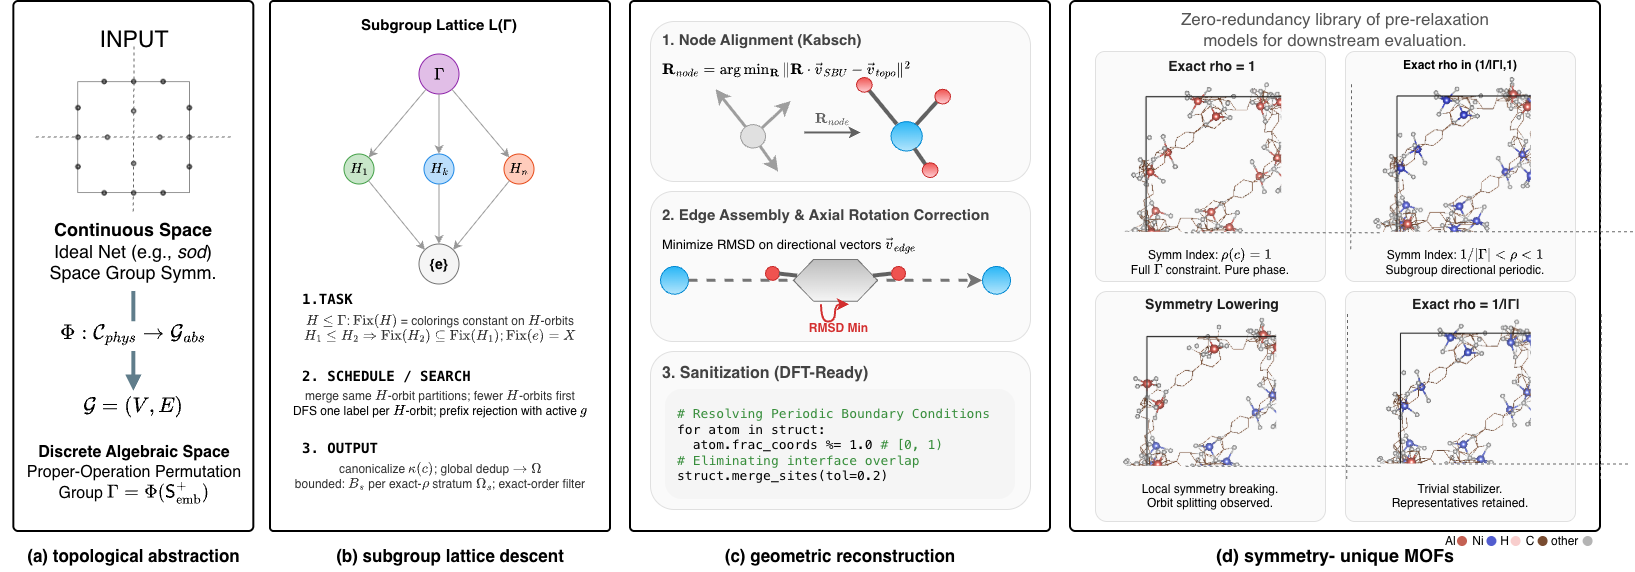
\includegraphics[width=\textwidth]{pipline.png}
    \caption{\textbf{Symmetry-aware candidate-generation pipeline.} The workflow reduces the periodic net to a quotient-graph representation, enumerates symmetry-distinct assignments under the proper-rotation group, and prepares the accepted assignments for reconstruction and downstream screening.}
    \label{fig:pipeline}
\end{figure}

\begin{algorithm}
\caption{Subgroup Lattice Descent}
\label{alg:enum}
\footnotesize
\begin{algorithmic}[1]
\Require Proper-rotation group $\Gamma$; vertex degrees $\{\deg(v)\}$; degree-typed ligand pools $\{\mathcal{C}_d\}$; degree counts $\{n_d\}$; optional task timeout $T_{\mathrm{task}}$; global cap $M_{\mathrm{total}}$; optional identity trigger $\Lambda_{\mathrm{id}}$ and identity cap $B_{\mathrm{id}}$
\Ensure Canonical representative set $\Omega$ with exact or partial Burnside report
\State initialize min-heap $Q$ keyed by orbit count; $\Omega \gets \emptyset$
\State push full-group task $\big(\mathcal{O}_{\Gamma},\,\infty\big)$ into $Q$
\For{each proper subgroup $H < \Gamma$ found from the subgroup lattice}
    \State compute $\mathcal{O}_H$ and its orbit-partition fingerprint
    \If{the fingerprint has not appeared before}
        \State push task $\big(\mathcal{O}_H,\,\infty\big)$ into $Q$
    \EndIf
\EndFor
\State $\mathcal{O}_{\{e\}} \gets \big\{\{v_1\},\dots,\{v_{|V|}\}\big\}$
\State estimate $\widehat{N}_{\mathrm{id}} \gets \text{naive-space} / |\Gamma|$
\State $b_{\mathrm{id}} \gets B_{\mathrm{id}}$ if $\widehat{N}_{\mathrm{id}} > \Lambda_{\mathrm{id}}$, else $\infty$
\State push identity task $\big(\mathcal{O}_{\{e\}},\,b_{\mathrm{id}}\big)$ into $Q$
\While{$Q$ is not empty}
    \State pop task $(\mathcal{O}, b)$ with smallest orbit count
    \State $s \gets |\Omega|$; deadline $\gets$ now $+\,T_{\mathrm{task}}$ if timeout is enabled
    \State \Call{CanonicalDFS}{$1,\; \langle \perp, \dots, \perp \rangle,\; \Gamma_{\mathrm{active}},\; \mathcal{O},\; b,\; s,\; \text{deadline}$}
\EndWhile
\State \Call{BurnsideReport}{$\Omega, \Gamma$} \Comment{exact closure or partial coverage}
\State \Return $\Omega$
\Statex
\Function{CanonicalDFS}{$k,\, c,\, \mathcal{A},\, \mathcal{O},\, b,\, s,\, \text{deadline}$}
    \If{deadline exceeded \textbf{ or } $|\Omega| \ge M_{\mathrm{total}}$ \textbf{ or } $|\Omega|-s \ge b$}
        \State \Return
    \EndIf
    \If{$k > |\mathcal{O}|$}
        \State $c^{\star} \gets \min_{g \in \Gamma} (g \cdot c)$
        \If{$c^{\star} \notin \text{Trie}$}
            \State insert $c^{\star}$; record $|\mathrm{Stab}_{\Gamma}(c^{\star})|$; $\Omega \gets \Omega \cup \{c^{\star}\}$
        \EndIf
        \State \Return
    \EndIf
    \State $d \gets \deg(\mathcal{O}_k)$
    \For{each $a \in \mathcal{C}_d$}
        \State assign $a$ to all vertices of $\mathcal{O}_k$
        \If{$\text{count}_d + |\mathcal{O}_k| > n_d$}
            \State undo $\mathcal{O}_k$; \textbf{continue}
        \EndIf
        \State $\mathcal{A}' \gets \emptyset$; $\;pruned \gets \textbf{false}$
        \For{each $g \in \mathcal{A}$}
            \If{$(g \cdot c) <_{lex} c$}
                \State $pruned \gets \textbf{true}$; \textbf{break}
            \ElsIf{$(g \cdot c) =_{lex} c$}
                \State $\mathcal{A}'.\text{add}(g)$
            \EndIf
        \EndFor
        \If{\textbf{not} $pruned$}
            \State \Call{CanonicalDFS}{$k+1,\, c,\, \mathcal{A}',\, \mathcal{O},\, b,\; s$}
        \EndIf
        \State undo assignment of $\mathcal{O}_k$
    \EndFor
\EndFunction
\end{algorithmic}
\end{algorithm}

\subsection*{From Enumerated Assignments to Crystal Models}
Turning an abstract assignment back into a crystal model is where orientation begins to matter. The quotient-graph assignment is first lifted back to the periodic net, and the unit-cell scale is set from the longest required connection length with a 5\% geometric buffer. Directionality is then recovered through two complementary reconstruction operations:
% 中文翻译：把抽象指派重新变回晶体模型时，取向问题才真正开始变得关键。我们首先将商图上的指派重新提升回周期性网络，并以所需连接长度中的最大值为基准、加入 5\% 的几何缓冲来设定晶胞尺度。随后，再通过两个互补的重构步骤恢复方向性：

\begin{enumerate}
\item \textbf{Node Alignment.} For each topological node, we collect the periodic connectivity vectors to all its neighbors.
The Kabsch algorithm then gives the optimal rotation matrix $\mathbf{R}_{node}$ for aligning the connection sites of the node SBU with these vectors, which fixes the spatial orientation of the SBU.
% 中文翻译：首先是“节点对齐”。对于每个拓扑节点，我们收集其与所有相邻节点之间的周期性连接向量。随后利用 Kabsch 算法求得最优旋转矩阵 $\mathbf{R}_{node}$，使节点构建单元（SBU）的连接位点与这些向量对齐，从而固定 SBU 的空间取向。

\item \textbf{Linker Placement.} For each edge in the graph, we compute the connection vector between two aligned nodes.
The algorithm retrieves the best-matching linker from the library, aligns it as a rigid body to this vector axis, and then refines its axial rotation by minimizing RMSD.
% 中文翻译：其次是“连接体放置”。对于图中的每条边，我们计算两个已对齐节点之间的连接向量。算法从库中检索最佳匹配的连接体，将其作为刚体对齐到该向量轴上，再通过最小化 RMSD 微调其绕轴旋转角度。
\end{enumerate}


The remaining reconstruction bookkeeping is less elegant but still essential. Periodic boundary mismatches are handled through coordinate normalization, lattice-aware edge adjustment, X-site fusion at a 0.8\,\AA\ tolerance, and a final merge of near-duplicate sites. Structures that pass the subsequent sanitization checks are retained as CP2K input geometries.
% 中文翻译：剩下的重构细节没有那么显眼，但同样关键。我们通过坐标归一化、考虑晶格周期性的边连接调整、0.8\,\AA\ 容差下的 X 位点融合，以及近重复位点的最终合并，来处理周期性边界错位问题。通过后续净化检查的结构会被保留为 CP2K 输入几何。

Every reconstructed candidate reported in this work goes through the same deterministic sequence: cell scaling, node alignment, linker placement, coordinate normalization, and sanitization.
% 中文翻译：本文报告的每个重构候选都经过同一套确定性流程：晶胞缩放、节点对齐、连接体放置、坐标归一化以及净化。

This reconstruction still makes one clear approximation: each building unit is treated as a rigid body, and its orientation is set by Kabsch alignment of its connection sites to the topological net. That description is reasonable for SBUs with well-defined connection geometry, such as paddlewheel, triangular-prismatic, and tetrahedral metal clusters. It is also reasonable for linkers whose internal degrees of freedom are either absent, such as BDC, BPDC, and imidazolates, or adequately represented by a single input conformer. It is not a conformational search. Linkers with rotatable bonds, such as alkoxy-functionalized or peptide-based linkers, are therefore represented one conformer at a time. The implications of this approximation are discussed further in Section~\ref{sec:limits}.
% 中文翻译：这一重构仍然建立在一个明确的近似之上：每个构建单元都被视为刚体，其取向通过将连接位点与拓扑网络进行 Kabsch 对齐来确定。对于具有明确连接几何的 SBU，如桨轮型、三棱柱型和四面体型金属簇，这样的处理是合理的。对于内部自由度要么不存在、如 BDC、BPDC、咪唑类，要么能够由单一输入构象充分代表的连接体，这样的处理同样合理。但它并不是构象搜索。对于含可旋转键的连接体，如烷氧基功能化或肽基连接体，当前做法只能按“每个输入构象返回一个结构”来处理。这一近似所带来的影响将在第~\ref{sec:limits}节进一步讨论。

\section*{Results}

\subsection*{Algebraic Correctness and External Cross-Check}
The enumeration stage was examined in three complementary ways. Exact-mode runs are checked first by Burnside closure, which confirms that the recovered representatives account for the full orbit space whenever the sum closes exactly. The same quotient-graph problems were then compared with CASM, and the comparison is summarized in Table~\ref{tab:casm}. For configuration spaces beyond the practical exhaustive range, we separately report bounded-regime behavior on \texttt{vba}, where truncation is intentional and the Burnside sum is read as a coverage diagnostic rather than a completeness proof.
% 中文翻译：这一枚举阶段通过三种互补方式进行考察。首先，对于精确模式运行，Burnside 闭合用于确认：只要求和能够精确闭合，所得代表元就覆盖了完整轨道空间。与此同时，我们还用 CASM 对同一批商图问题进行了比较，结果汇总见表~\ref{tab:casm}。而对于超出实际可穷举范围的构型空间，我们则单独报告 \texttt{vba} 上的受限运行行为；在这种情形下，截断是有意为之的，Burnside 求和应被读作覆盖诊断，而不是完备性证明。

Two different roles need to be distinguished in that table. The exhaustive \texttt{ffc} cases are direct correctness cross-checks: after the two group actions are reconciled, they reproduce the same proper-rotation counts on both sides. The larger \texttt{fjh} rows serve a different purpose. There, our enumerator is run in exhaustive mode, whereas CASM is reported from matched bounded runs on the same quotient graph. Those rows therefore show how coverage diverges within a practical runtime window once the space becomes large; they are not the primary correctness evidence for the algebraic stage.
% 中文翻译：这张表里需要区分两种不同的作用。可穷举的 \texttt{ffc} 算例是直接的正确性交叉核对：在对两种群作用完成对账之后，双方给出了相同的真旋转计数。更大的 \texttt{fjh} 行承担的则是另一项任务。在这些行中，我方枚举器以可穷举模式运行，而 CASM 报告的是同一商图上匹配运行窗口下的受限结果。因此，这些行展示的是：当空间变大后，覆盖率如何在实际运行窗口内出现分化；它们并不是代数阶段最主要的正确性证据。

\begin{table}[htbp]
\centering
\scriptsize
\setlength{\tabcolsep}{1.0mm}
\renewcommand{\arraystretch}{1.2}
\caption{Cross-check against CASM on identical quotient graphs. The \texttt{ffc} rows are exhaustive comparisons on both sides and serve as the direct correctness cross-checks. The larger \texttt{fjh} rows use our enumerator in exhaustive mode, while CASM is reported from matched bounded runs on the same quotient graph; those rows therefore illustrate coverage differences within a practical runtime window rather than a disagreement in exact orbit counting. ``Orbits ($\Gamma$)'' is the proper-rotation count $P$ from our enumerator. ``CASM'' is the raw count $F_{\mathrm{total}}$ modulo the complete crystallographic factor group. The full-group count is reconciled to the proper-rotation count by $P=A+2C$. Times are single-core wall-clock values for the enumeration core only (median of three runs).}
\label{tab:casm}
\begin{tabular}{llccccc}
\toprule
\textbf{Topology} & \textbf{Ligand pool} & \textbf{Naive} & \textbf{Orbits ($\Gamma$)} & \textbf{CASM} & \textbf{Undercount} & \textbf{Time ratio (s)} \\
\midrule
\texttt{ffc} & $|\mathcal{C}_3|{=}2,|\mathcal{C}_4|{=}2$ & $1.28\times10^{2}$ & 42      & 42      & 0\%  & $0.098 / 1.5\!\times\!10^{-4}$ \\
\texttt{ffc} & $|\mathcal{C}_3|{=}3,|\mathcal{C}_4|{=}3$ & $2.19\times10^{3}$ & 513     & 513     & 0\%  & $0.100 / 1.7\!\times\!10^{-3}$ \\
\midrule
\texttt{fjh} & $|\mathcal{C}_3|{=}1,|\mathcal{C}_4|{=}2$ & $4.10\times10^{3}$ & 394     & 265     & 33\% & $0.194 / 3.3\!\times\!10^{-3}$ \\
\texttt{fjh} & $|\mathcal{C}_3|{=}2,|\mathcal{C}_4|{=}1$ & $6.55\times10^{4}$ & 4{,}756 & 2{,}476 & 48\% & $0.291 / 0.057$ \\
\texttt{fjh} & $|\mathcal{C}_3|{=}1,|\mathcal{C}_4|{=}3$ & $5.31\times10^{5}$ & 36{,}369& 20{,}655& 43\% & $2.12 / 0.402$ \\
\bottomrule
\end{tabular}
\end{table}

The bounded regime needs a different interpretation. Once the estimated orbit count crosses the identity-trigger threshold, the run is no longer used as a correctness cross-check against CASM. Instead, Table~\ref{tab:bounded} reports representative \texttt{vba} cases in which the current safeguards intentionally stop the search before full-space closure. The truncation itself is not arbitrary: the scheduler first processes the full-group and proper-subgroup tasks, and only then enters the identity tail that dominates the orbit count. In that sense, the bounded prefix remains informative rather than merely incomplete, because it preferentially retains the more symmetry-structured part of the search space before cutting into the large asymmetric remainder. These rows should therefore be read as partial-coverage diagnostics for large spaces, not as exhaustive orbit counts.
% 中文翻译：受限运行区间需要按另一种方式来解读。一旦估算轨道数超过恒等层触发阈值，这类运行就不再被用作与 CASM 的正确性交叉核对。相反，表~\ref{tab:bounded} 报告的是若干代表性的 \texttt{vba} 算例：在这些大空间里，当前保护机制会有意在全空间闭合之前停止搜索。这里的截断并不是任意发生的：调度器会先处理 full-group 和 proper-subgroup 任务，之后才进入通常主导轨道数的 identity 尾部。因此，这样得到的受限前缀并不只是一个“不完整子集”，而是会优先保留搜索空间中对称性结构更强的那一部分，再切掉庞大的低对称尾部。故这些行应被读作大空间下的部分覆盖诊断，而不是可穷举轨道总数。

\begin{table}[htbp]
\centering
\small
\caption{\textbf{Bounded-regime behavior beyond the practical exhaustive range.} These \texttt{vba} rows are not CASM cross-checks. They document the operational behavior of the enumerator once the run is intentionally truncated by the current safeguards. The reported coverages are the Burnside-based covered fractions at termination and therefore quantify partial rather than exhaustive enumeration.}
\label{tab:bounded}
\setlength{\tabcolsep}{2.6mm}
\renewcommand{\arraystretch}{1.2}
\begin{tabular}{lclcc}
\toprule
\textbf{Topology} & \textbf{Ligand pool} & \textbf{Naive space} & \textbf{Returned orbits} & \textbf{Time (s)} \\
\midrule
\texttt{vba} & $|\mathcal{C}_4|{=}2$ & $4.29\times10^{9}$  & 131{,}864 $(0.026\%)$    & 8.68 \\
\texttt{vba} & $|\mathcal{C}_4|{=}3$ & $1.85\times10^{15}$ & 500{,}000 $(<0.001\%)$ & 30.37 \\
\bottomrule
\end{tabular}
\end{table}
\subsection*{Geometric Instantiation Across Representative Topologies}
\label{sec:validation}

% 中文翻译（表注）：在相同商图上与 CASM 的交叉检查。\texttt{ffc} 行对应双方都可穷举的比较；更大的 \texttt{fjh} 行则使用我方枚举器的可穷举结果，并将 CASM 在相同商图上的匹配受限运行结果一并报告，因此这些行反映的是实际运行窗口内的覆盖差异，而不是全空间分歧。“Orbits (Γ)”为我方枚举器给出的真旋转计数 $P$；“CASM”为按完整晶体学因子群取模得到的原始计数 $F_{\mathrm{total}}$。完整群计数通过 $P=A+2C$ 与真旋转计数对账。时间为单核、仅枚举核心的墙钟中位数。

We then tested whether the accepted assignments survive oriented reconstruction as usable periodic frameworks. Across the representative \texttt{ffc}, \texttt{fjh}, \texttt{vba}, \texttt{hwx}, and \texttt{nbo} topologies, the same Phase~III protocol produced sanitizable periodic CIF models whose recovered building-unit orientations remained compatible with the intended topological skeletons. In the sampled \texttt{ffc} and \texttt{fjh} subsets, the reconstruction audit returned sanitizable CIFs for every sampled candidate. What varied from one topology to another was the rate of topology recovery after sanitization, and steric clashes were still common before relaxation. Representative reconstructed models are shown in Fig.~\ref{fig:reconstruction_gallery}.
% 中文翻译：随后我们检验，被接受的指派在经过取向重构之后能否作为可用的周期性框架保留下来。对于代表性的 \texttt{ffc}、\texttt{fjh}、\texttt{vba}、\texttt{hwx} 和 \texttt{nbo} 拓扑，同一套第三阶段流程都生成了可通过净化的周期性 CIF 模型，且恢复得到的构建单元取向与目标拓扑骨架保持一致。在抽样的 \texttt{ffc} 和 \texttt{fjh} 子集中，重构审计对全部候选都返回了可净化的 CIF。不同拓扑之间真正变化的是净化之后的拓扑恢复率，而在弛豫之前立体碰撞仍然较为常见。代表性的重构模型见图~\ref{fig:reconstruction_gallery}。


\begin{figure}[htbp]
    \centering
    \begin{subfigure}[t]{0.32\linewidth}
        \centering
        \includegraphics[width=\linewidth]{reconstruction_gallery/ffc_panel.png}
        \caption*{\texttt{ffc}}
    \end{subfigure}
    \hfill
    \begin{subfigure}[t]{0.32\linewidth}
        \centering
        \includegraphics[width=\linewidth]{reconstruction_gallery/fjh_panel.png}
        \caption*{\texttt{fjh}}
    \end{subfigure}
    \hfill
    \begin{subfigure}[t]{0.32\linewidth}
        \centering
        \includegraphics[width=\linewidth]{reconstruction_gallery/vba_panel.png}
        \caption*{\texttt{vba}}
    \end{subfigure}

    \vspace{0.4em}

    \begin{minipage}{0.76\linewidth}
    \centering
    \begin{subfigure}[t]{0.42\linewidth}
        \centering
        \includegraphics[width=\linewidth]{reconstruction_gallery/hwx_panel.png}
        \caption*{\texttt{hwx}}
    \end{subfigure}
    \hfill
    \begin{subfigure}[t]{0.42\linewidth}
        \centering
        \includegraphics[width=\linewidth]{reconstruction_gallery/nbo_panel.png}
        \caption*{\texttt{nbo}}
    \end{subfigure}
    \end{minipage}
    \caption{Representative crystal models reconstructed from symmetry-distinct assignments on five topologies: \texttt{ffc}, \texttt{fjh}, \texttt{vba}, \texttt{hwx}, and \texttt{nbo}. Each panel shows a sanitizable periodic CIF obtained after rigid-body placement of the selected building units on the target net.}
    % 中文翻译：由五种拓扑上的对称互异指派重构得到的代表性晶体模型。图中展示了 \texttt{ffc}、\texttt{fjh}、\texttt{vba}、\texttt{hwx} 和 \texttt{nbo} 五种拓扑对应的可净化周期性 CIF，它们均由所选构建单元在目标网络上的刚体放置得到。该图的重点在于说明：从抽象指派到原子级晶体模型的过渡能够在不同网络几何中稳定完成。
    \label{fig:reconstruction_gallery}
\end{figure}


\subsection*{Illustrative Screening-Stage DFT Example}

To see how the generated and reconstructed candidates behave in a downstream screen, we evaluated single-point DFT energies for a bounded set of rigidly assembled structures within fixed chemical compositions. Each comparison keeps the building-block inventory unchanged, so the resulting energy differences can be read on the same assembled-geometry basis. We did not relax these structures, because relaxation would move the comparison onto a different geometric footing.
% 中文翻译：为了看清生成并重构得到的候选在下游筛选中会如何表现，我们在一个有边界的固定组成样本上，对刚性组装得到的结构进行了单点 DFT 计算。每一组比较都保持构建单元配方不变，因此得到的能量差异可以放在同一组装几何基准上来解读。这里不进行结构弛豫，因为一旦弛豫，这种比较所依赖的几何基准也会随之改变。

For the smaller \texttt{ffc} topology, 21 converged calculations span eight fixed-composition groups. Figure~\ref{fig:symmetry_screening}(a) shows the overall spread of sampled energies, and Fig.~\ref{fig:symmetry_screening}(b) resolves the same structures within fixed-composition groups. Under the operational bins low $[0,0.25)$, medium $[0.25,0.75]$, and high $(0.75,1]$, the composition-wise minimum falls in the medium- or high-symmetry strata in all eight groups. In this sampled \texttt{ffc} set, the low-energy candidates therefore remain in the medium- and high-symmetry part of the search order.
% 中文翻译：对于较小的 \texttt{ffc} 拓扑，当前共有 21 个已收敛计算，分布在 8 个固定组成组中。图~\ref{fig:symmetry_screening}(a) 展示了采样能量的整体分布，而图~\ref{fig:symmetry_screening}(b) 则把同一批结构放回固定组成组内来观察。在本文采用的操作性区间划分，即低对称 $[0,0.25)$、中对称 $[0.25,0.75]$、高对称 $(0.75,1]$ 下，8 个组成组的组内最低能点全部落在中对称或高对称层级。因此，在当前采样到的 \texttt{ffc} 集合中，低能候选保留在搜索顺序的中高对称部分。

The larger \texttt{fjh} topology gives a finer fixed-composition test because both sampled compositions resolve five distinct $\rho$ strata. In the fully sampled \texttt{comp\_a} set, 16 converged calculations cover all five symmetry levels, and the minimum appears at $\rho=0.5$. In the equally complete \texttt{comp\_b} set, 16 converged calculations again cover all five levels, and the minimum appears at $\rho=1.0$. Read together with the \texttt{ffc} comparison, these two fixed-composition tests show that symmetry-prioritized traversal still retains competitive low-energy candidates in the sampled screening space~\cite{peng2024learning,zeni2023mattergen,okabe2025structural}.
% 中文翻译：较大的 \texttt{fjh} 拓扑提供了更细致的固定组成检验，因为当前采样到的两个组成都能分辨出 5 个不同的 $\rho$ 层级。在完整采样的 \texttt{comp\_a} 集合中，16 个已收敛计算覆盖了全部 5 个对称性层级，最低能点出现在 $\rho=0.5$。在同样完整的 \texttt{comp\_b} 集合中，16 个已收敛计算也覆盖了全部 5 个层级，最低能点则出现在 $\rho=1.0$。把它们与 \texttt{ffc} 的比较一起看，可以得到一个更直接的结论：在当前采样到的筛选空间内，对称性优先遍历仍然能够保留有竞争力的低能候选~\cite{peng2024learning,zeni2023mattergen,okabe2025structural}。


\begin{figure}[htbp]
    \centering
    \begin{subfigure}[t]{0.495\linewidth}
        \centering
        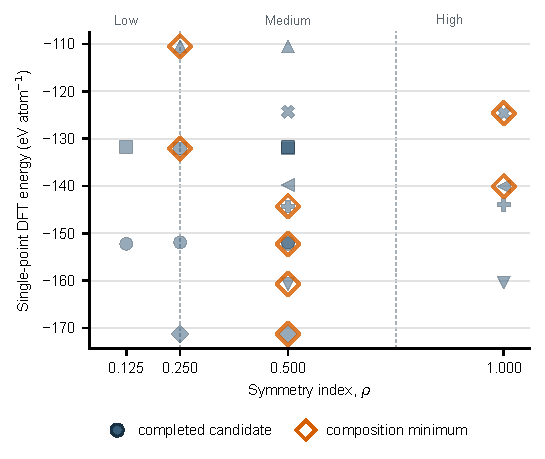
\includegraphics[width=\linewidth]{ffc_pooled_symmetry_energy_a.pdf}
        \caption{Pooled single-point energies for the \texttt{ffc} set.}
    \end{subfigure}
    \hfill
    \begin{subfigure}[t]{0.495\linewidth}
        \centering
        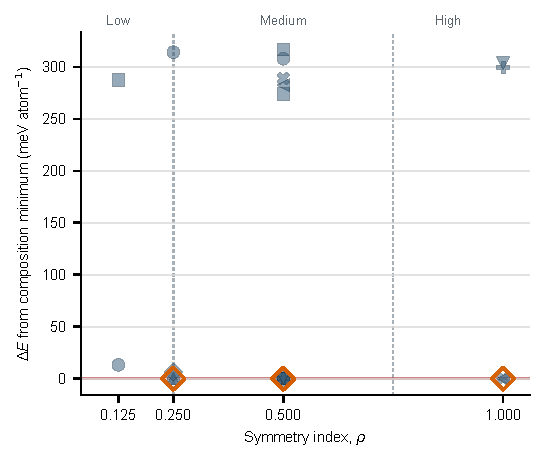
\includegraphics[width=\linewidth]{ffc_pooled_symmetry_energy_b.pdf}
        \caption{Composition-controlled $\Delta E$ for the same \texttt{ffc} candidates.}
    \end{subfigure}
    
    \vspace{0.5em}

    \begin{subfigure}[t]{0.495\linewidth}
        \centering
        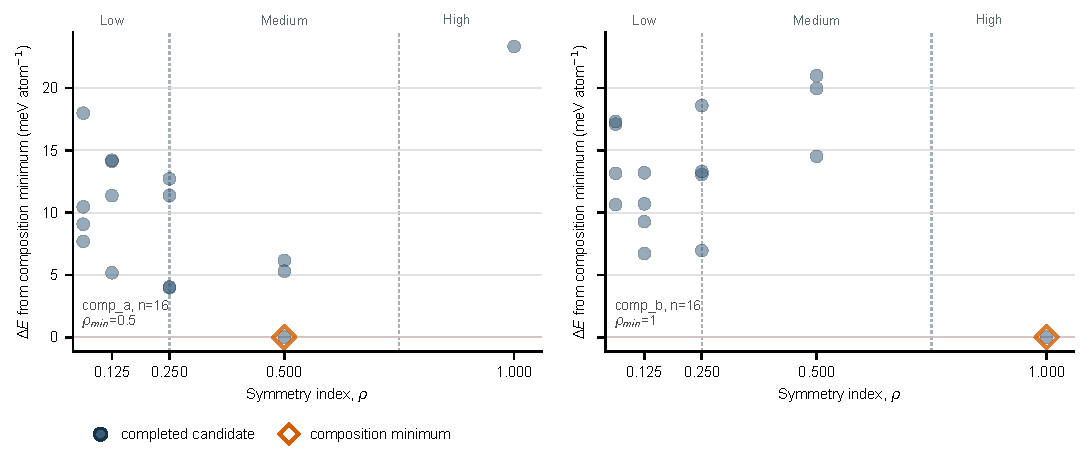
\includegraphics[width=\linewidth,trim={0 0 262 0},clip]{fjh_dual_delta_symmetry_energy.pdf}
        \caption{\texttt{fjh comp\_a} composition-controlled $\Delta E$.}
    \end{subfigure}
    \hfill
    \begin{subfigure}[t]{0.495\linewidth}
        \centering
        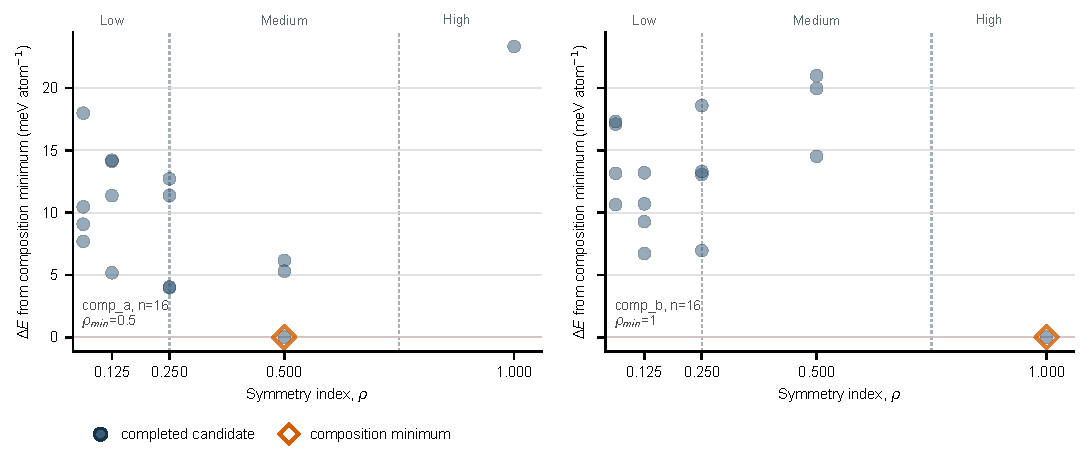
\includegraphics[width=\linewidth,trim={262 0 0 0},clip]{fjh_dual_delta_symmetry_energy.pdf}
        \caption{\texttt{fjh comp\_b} composition-controlled $\Delta E$.}
    \end{subfigure}
\caption{Illustrative single-point DFT screening results across two topology scales. Filled markers denote converged candidates and open markers denote the minimum within each fixed-composition comparison set. Panels (a,b) show the pooled energies and composition-controlled $\Delta E$ analysis for the multi-composition \texttt{ffc} set. Panels (c,d) show composition-controlled $\Delta E$ for the fully sampled \texttt{fjh comp\_a} and \texttt{fjh comp\_b} sets.}
% 中文翻译：两种拓扑尺度下的说明性单点 DFT 筛选结果。实心标记表示已收敛候选，空心标记表示各固定组成比较集合中的最低能点。子图 (a,b) 展示多组成 \texttt{ffc} 集合的汇总能量与固定组成 $\Delta E$ 分析。子图 (c,d) 展示完整采样的 \texttt{fjh comp\_a} 与 \texttt{fjh comp\_b} 集合在固定组成条件下的 $\Delta E$ 结果。
    \label{fig:symmetry_screening}
\end{figure}



\section*{Discussion}
\label{sec:discussion}
At the scale studied here, the main value of the workflow is that it keeps candidate generation, reconstruction, and screening-stage evaluation on a consistent symmetry-aware footing even though they are carried out as separate stages. The enumeration step removes redundant assignments before they propagate downstream. The reconstruction step then tests whether those assignments can actually be carried forward as periodic crystal models with explicit building-unit orientation. The result is a candidate set that is smaller, structurally interpretable, and directly usable for the next stage of analysis.
% 中文翻译：在本文考察的尺度上，这一工作流程的主要价值在于：尽管候选生成、重构和筛选阶段评估是分阶段执行的，它们仍始终建立在同一套一致的对称性感知框架之上。枚举步骤在候选向下游传播之前就去除了冗余指派。随后，重构步骤进一步检验这些指派能否真正以具有显式构建单元取向的周期性晶体模型形式被保留下来。由此得到的是一组规模更小、结构上更易解释、也能直接进入下一阶段分析的候选集合。

The validation results support that interpretation in a bounded way. Exact-mode algebraic checks establish that the proper-rotation quotient is handled consistently in the exhaustive cases, while the \texttt{vba} stress test shows how the same ordering behaves once truncation becomes unavoidable. The reconstruction tests show that sampled candidates can be converted into sanitizable periodic models, but also that topology recovery remains topology-dependent and steric cleanup is still left to later relaxation. The DFT comparisons then serve only as illustrative screening-stage examples for the same candidate set: within the sampled fixed-composition spaces, the composition-controlled comparisons indicate that symmetry-prioritized traversal continues to retain competitive low-energy structures, but they do not constitute an independent materials finding. Together, these results support the method as a crystal-engineering route to candidate preparation and early-stage evaluation.
% 中文翻译：现有验证结果以一种有边界的方式支撑了上述解释。精确模式下的代数核对说明，在可穷举算例中，真旋转取商的处理是自洽的，而 \texttt{vba} 的压力测试则展示了当截断不可避免时，同样的排序策略会如何表现。重构测试表明，抽样候选能够被转化为可净化的周期性模型，但同时也说明：拓扑恢复仍然具有明显的拓扑依赖性，而立体清理则仍需留待后续弛豫。DFT 比较则仅作为同一组候选进入筛选阶段的说明性示例：在当前采样到的固定组成空间里，组成受控比较表明对称性优先遍历仍能保留有竞争力的低能结构，但它们并不构成独立的材料发现。综合来看，这些结果支持将该方法视为一条面向晶体工程的候选准备与早期评估路径。

\subsection*{Current Limits of the Validation}
\label{sec:limits}
The main limit lies in the rigid-body reconstruction itself. The present implementation assumes that node SBUs and linkers can be placed as rigid units once their connection geometry is specified. That approximation is reasonable for many rigid or semi-rigid building blocks, but it does not cover highly flexible linkers whose placement would need to be coupled to conformational search. The current reconstruction stage therefore tests geometric compatibility on a fixed conformer basis rather than the full conformational landscape available to a flexible framework. A second limit is interpretive rather than geometric: the DFT results reported here are single-point scores on as-assembled structures and are intended only for fixed-composition screening-stage comparisons, not for final thermodynamic ranking across chemistries.
% 中文翻译：当前最主要的限制来自刚体重构本身。当前实现假定，只要连接几何被给定，节点 SBU 和连接体就可以作为刚性单元被放置。这一近似对许多刚性或半刚性的构建单元是合理的，但对于高度柔性的连接体并不适用，因为那类体系的放置需要与构象搜索耦合。也就是说，当前重构阶段检验的是固定输入构象条件下的几何兼容性，而不是柔性框架可能涉及的完整构象图景。第二个限制并不在几何层面，而在解释层面：本文报告的 DFT 结果是基于组装初始结构的单点打分，其用途仅限于固定组成条件下的筛选阶段比较，而不是跨不同 chemistry 的最终热力学排序。

\section*{Methods}
\subsection*{Computational Details}
The framework is implemented in Python 3.8 and follows the same three-stage sequence used in the main text: symmetry extraction on the periodic net, symmetry-distinct enumeration on the quotient graph, and rigid-body reconstruction of the accepted assignments.
% 中文翻译：该框架基于 Python 3.8 实现，并遵循与正文一致的三阶段顺序：在周期性网络上提取对称性、在商图上进行对称互异枚举，以及对被接受指派执行刚体重构。

In Phase I (Abstraction), \texttt{pymatgen} is used for crystallographic symmetry analysis. We scan \texttt{symprec} $\in \{0.01, 0.1, 0.3\}$\,\AA\ to identify a robust set of symmetry operations, which are then projected onto graph automorphism groups.
% 中文翻译：在第一阶段（抽象）中，我们使用 \texttt{pymatgen} 进行晶体学对称性分析。通过扫描 \texttt{symprec} $\in \{0.01, 0.1, 0.3\}$\,\AA，我们鲁棒地识别对称操作集合，并随后将其投影为图自同构群。

In Phase II (Enumeration), we handle degree-constrained spaces of up to $\sim\!5\times10^{5}$ configurations in the benchmark cases summarized in Table~\ref{tab:casm}. Proper subgroups are enumerated through a SymPy-based lattice walk, with a cyclic-subgroup fallback if that step fails. Orbit calculations, canonical-form checks, and duplicate removal are carried out with data structures chosen for compact storage and stable performance, while the implementation also supports optional operational safeguards such as per-task timeouts and global result caps.
% 中文翻译：在第二阶段（枚举）中，我们在表~\ref{tab:casm} 汇总的基准算例里处理至多约 $\sim\!5\times10^{5}$ 个构型的度数约束空间。真子群的遍历通过基于 SymPy 的子群格搜索完成；若该步骤失败，则退化为循环子群回退路径。轨道计算、正则形检查和重复去除均通过适合这些搜索空间的紧凑型数据结构完成，以保持稳定性能；与此同时，该实现还支持可选的运行保护措施，例如按任务设置的超时和全局结果数上限。

In Phase III (Reconstruction), the Kabsch algorithm is implemented through singular value decomposition in \texttt{NumPy} to compute RMSD-minimizing rotation matrices. The assembled structure then undergoes secondary symmetry analysis (\texttt{symprec}=0.3\,\AA) to recover the nominal space group while tolerating minor distortions introduced during rigid-body placement.
% 中文翻译：在第三阶段（重构）中，Kabsch 算法通过 \texttt{NumPy} 中的奇异值分解实现，用于计算最小化 RMSD 的旋转矩阵。组装后的结构随后进行二次对称性分析（\texttt{symprec}=0.3\,\AA），以在容许刚体放置引入微小畸变的情况下恢复标称空间群。

The reconstruction stage follows the same ordered sequence used in the main text: graph enrichment, rigid-body placement of nodes and linkers, periodic coordinate normalization, and sanitization before any structure is passed to downstream screening.
% 中文翻译：重构阶段按照与正文一致的固定顺序执行，即图信息增强、节点与连接体的刚体放置、周期性坐标归一化，以及在任何结构进入后续筛选前完成净化。

All computations were executed on a single-core Intel Core i5 processor.
% 中文翻译：所有计算均在单核 Intel Core i5 处理器上执行。

\subsection*{CASM Comparison Protocol}

Cross-validation uses \textsf{libcasm-configuration}~2.3.1 and \textsf{libcasm-xtal}~2.3.0 under Python~3.11 (Algorithm~\ref{alg:casm}). The worker presents CASM with the same degree-constrained space traversed by our enumerator, with each site carrying the occupant set fixed by its coordination number. A run is accepted only if the proper-rotation subgroup of the resulting factor group attains the order $|\Gamma|$ shared by both codes. Enumeration over the primitive supercell then yields one representative per full-group orbit, which is reconciled to the proper-rotation count $P=A+2C$ and checked against our result. For comparable timings, each case is enumerated in an isolated single-threaded subprocess and reported as the median of three runs. The \texttt{vba} pools are placed under a watchdog that declares the run intractable once it exceeds the wall-clock or memory limit.
% 中文翻译：交叉验证在 Python~3.11 下使用 \textsf{libcasm-configuration}~2.3.1 和 \textsf{libcasm-xtal}~2.3.0 执行（算法~\ref{alg:casm}）。worker 向 CASM 提供与本文枚举器相同的度数约束空间，每个位点携带由其配位数决定的占据集合。仅当所得因子群的真旋转子群达到两种代码共享的阶 $|\Gamma|$ 时，才接受该次运行。随后在初基超胞上枚举，为每个全群轨道产生一个代表元，并将其对账为真旋转计数 $P=A+2C$ 后与本文结果比较。为使计时可比，每个算例均在隔离的单线程子进程中枚举，并报告三次运行的中位数。\texttt{vba} 配体池由看门狗监控，一旦超过墙钟或内存限制即判定为不可处理。

\begin{algorithm}[h]
\caption{CASM cross-validation for one (topology $\tau$, ligand pool)}
\label{alg:casm}
\begin{algorithmic}[1]
\Procedure{Worker}{$\tau,\,|\mathcal{C}_3|,\,|\mathcal{C}_4|$}\Comment{python3.11; libcasm}
  \State match CIF sites to graph nodes $v_i$ ($\lVert\Delta\mathrm{frac}\rVert<10^{-3}$)
  \State $\mathrm{occ}(s_i)\gets$ $|\mathcal{C}_3|$ labels if $\deg v_i{=}3$ else $|\mathcal{C}_4|$ labels
  \State $\textsc{Prim}\gets\textsc{BuildPrim}(\text{lattice},\{\mathrm{frac}(s_i)\},\mathrm{occ})$
  \State $\Gamma_{\!c}\gets\{g\in\textsc{FactorGroup}(\textsc{Prim}):\det g>0\}$
  \State \textbf{abort if} $|\Gamma_{\!c}|\neq|\Gamma|$\Comment{proper symmetry must match}
  \State $t_0\gets\textsc{Clock}();\ F\gets 0$\Comment{time enumeration only}
  \For{$c\in\textsc{ConfigEnumAllOccupations}(\textsc{Prim},\text{vol-1 cell})$}
    \State $F\gets F+1$\Comment{one rep per full-group orbit}
  \EndFor
  \State \Return $F,\ \textsc{Clock}()-t_0,\ \text{peak RSS}$
\EndProcedure
\Statex
\Procedure{Compare}{$\tau,\,|\mathcal{C}_3|,\,|\mathcal{C}_4|,\,P$}\Comment{$P$ from our enumerator}
  \For{$r\gets 1$ to $3$}
    \State run \textsc{Worker} in a fresh single-thread subprocess
    \State \textbf{if} $\tau=\texttt{vba}$: kill as intractable if $t>30$\,min or RSS$>8$\,GB
  \EndFor
  \State $(F,t,\text{mem})\gets$ median-wall-clock run
  \State $C\gets P-F;\quad A\gets 2F-P$\Comment{$F{=}A{+}C,\ P{=}A{+}2C$}
  \State \textbf{assert} $A\ge0\wedge C\ge0$
  \State \Return $F,\ P,\ t,\ \text{mem}$
\EndProcedure
\end{algorithmic}
\end{algorithm}

\subsection*{DFT Energy Validation}
Single-point energies were computed with CP2K/Quickstep~\cite{cp2k2020} using the Gaussian--plane-wave method at the PBE+D3 level~\cite{perdew1996pbe,grimme2010d3}. Calculations used DZVP-MOLOPT-PBE-GTH basis sets and GTH pseudopotentials. Plane-wave and relative cutoffs were set to 500 and 60\,Ry, respectively.
% 中文翻译：单点能通过 CP2K/Quickstep~\cite{cp2k2020} 的 Gaussian--plane-wave 方法在 PBE+D3 水平下计算~\cite{perdew1996pbe,grimme2010d3}。计算采用 DZVP-MOLOPT-PBE-GTH 基组和 GTH 赝势。平面波截断能和相对截断能分别设为 500 和 60\,Ry。

Because the frameworks combine transition metals with conjugated linkers, they have small HOMO--LUMO gaps. The orbital-transformation SCF scheme therefore did not converge reliably. We used traditional diagonalization with Fermi--Dirac smearing, an electronic temperature of 300\,K, 30 added molecular orbitals, and Broyden charge mixing. The SCF settings were $\mathrm{EPS\_SCF}=5\times10^{-5}$ with a 300-step ceiling.
% 中文翻译：由于这些框架同时包含过渡金属和共轭连接体，其 HOMO--LUMO 能隙较小。因此，轨道变换 SCF 方案难以稳定收敛。我们采用传统对角化，并结合 Fermi--Dirac 展宽、300\,K 电子温度、30 个附加分子轨道和 Broyden 电荷混合。SCF 设置为 $\mathrm{EPS\_SCF}=5\times10^{-5}$，最大步数为 300。

The DFT protocol is included as an illustrative connection between enumeration/reconstruction and downstream screening on rigidly assembled, as-enumerated geometries. Each candidate was scored at the single-point level while keeping graph connectivity and initial placement fixed across symmetry classes, so the comparison probes whether symmetry-prioritized traversal retains promising candidates on a common assembled-geometry manifold. Any retention inference is drawn only from fixed-composition comparisons on that common manifold. The reported energies are therefore geometry-consistent screening scores tied to this stage of the method. Final thermodynamic ranking requires subsequent geometry relaxation.
% 中文翻译：该 DFT 协议被纳入本文，是为了说明枚举/重构结果如何衔接到刚性组装、保持枚举初始几何的下游筛选流程。每个候选都在保持不同对称性类别之间图连接关系和初始放置方式一致的前提下进行单点打分，因此该比较检验的是：在共同的组装几何流形上，对称性优先遍历是否能够保留有前景的候选。关于保留效应的所有推论，都只来自这一共同流形上的固定组成比较。因此，本文报告的能量是与该方法这一阶段对应的几何一致筛选分数。最终热力学排序仍需要后续几何弛豫。

To reduce chemical-composition bias, energy comparisons were made within fixed compositions. The \texttt{ffc} validation contains 21 converged single-point calculations across eight composition groups and is used as a multi-composition retention test under changing chemical inventory. Its pooled energy view is retained only as a descriptive display, whereas the composition-controlled comparisons provide the interpretive basis. The \texttt{fjh} validation is used differently: within the fully sampled \texttt{comp\_a} and \texttt{comp\_b} subsets, 32 converged structures cover all five symmetry strata in two independent fixed-composition tests. We therefore use \texttt{ffc} and \texttt{fjh} as complementary validation modes under one protocol, rather than as interchangeable measurements of a single trend.
% 中文翻译：为降低化学组成偏差，能量比较在固定组成内部进行。\texttt{ffc} 验证包含 8 个组成组中的 21 个已收敛单点能计算，并被用作在化学配方变化条件下的跨组成保留效应检验。其中，汇总能量视图只保留为描述性展示，而真正承担解释功能的是组成受控比较。\texttt{fjh} 验证的作用则不同：在完整采样的 \texttt{comp\_a} 和 \texttt{comp\_b} 子集中，共有 32 个已收敛结构，分别在两个独立的固定组成测试中覆盖了全部 5 个对称性层级。因此，本文将 \texttt{ffc} 和 \texttt{fjh} 视为在同一协议下的两种互补验证模式，而不是对同一趋势的可互换测量。

\section*{Data Availability}
The source code for the self-verifying enumeration framework and the benchmark experiments is available on GitHub at \url{https://github.com/ttttxx/Symmetry-Aware-Enumeration-of-mof.git}. The repository also contains the topology and structure inputs used for enumeration under the \texttt{data/} directories, the reconstruction-gallery assets and figure-preparation script used for Fig.~\ref{fig:reconstruction_gallery} under \texttt{paper/}, and the DFT selection records and analysis outputs used for Fig.~\ref{fig:symmetry_screening} under \texttt{results/dft\_validation/}. These materials include the reported source CIF files, representative generated CIF models, the \texttt{selected\_structures.json} screening record, and the plotting scripts needed to regenerate the manuscript figures.
% 中文翻译：自验证枚举框架和基准实验的源代码可在 GitHub 获取：\url{https://github.com/ttttxx/Symmetry-Aware-Enumeration-of-mof.git}。仓库还包含用于枚举的拓扑与结构输入（位于 \texttt{data/} 目录）、用于图~\ref{fig:reconstruction_gallery} 的重构图库素材与制图脚本（位于 \texttt{paper/} 目录），以及用于图~\ref{fig:symmetry_screening} 的 DFT 结构选择记录和分析输出（位于 \texttt{results/dft\_validation/} 目录）。这些材料包括文中使用的源 CIF 文件、代表性的生成 CIF 模型、\texttt{selected\_structures.json} 筛选记录，以及重现正文图件所需的绘图脚本。


\section*{Acknowledgements}
Funding information will be added before submission.
% 中文翻译：资助信息将在投稿前补充。

\section*{Author Contributions}
H.L. conceived the study; H.L. and J.T. developed the algorithm and performed the experiments; all authors discussed results and contributed to the manuscript.
% 中文翻译：H.L. 构思了本研究；H.L. 和 J.T. 开发了算法并进行了实验；所有作者讨论了结果并共同撰写了手稿。

\section*{Competing Interests}
The authors declare no competing interests
% 中文翻译：作者声明不存在利益冲突。
%%===========================================================================================%%

\newpage
\clearpage
\section*{Reference}

\bibliography{reference}

\end{document}
